%% This is file `elsarticle-template-1-num.tex',
%%
%% Copyright 2009 Elsevier Ltd
%%
%% This file is part of the 'Elsarticle Bundle'.
%% ---------------------------------------------
%%
%% It may be distributed under the conditions of the LaTeX Project Public
%% License, either version 1.2 of this license or (at your option) any
%% later version.  The latest version of this license is in
%%    http://www.latex-project.org/lppl.txt
%% and version 1.2 or later is part of all distributions of LaTeX
%% version 1999/12/01 or later.
%%
%% Template article for Elsevier's document class `elsarticle'
%% with numbered style bibliographic references
%%
%% $Id: elsarticle-template-1-num.tex 149 2009-10-08 05:01:15Z rishi $
%% $URL: http://lenova.river-valley.com/svn/elsbst/trunk/elsarticle-template-1-num.tex $
%%
\documentclass[preprint,12pt]{elsarticle}

\usepackage[colorlinks]{hyperref}
\usepackage[colorinlistoftodos]{todonotes}
\usepackage{verbatim}

%% Use the option review to obtain double line spacing
%% \documentclass[preprint,review,12pt]{elsarticle}

%% Use the options 1p,twocolumn; 3p; 3p,twocolumn; 5p; or 5p,twocolumn
%% for a journal layout:
%% \documentclass[final,1p,times]{elsarticle}
%% \documentclass[final,1p,times,twocolumn]{elsarticle}
%% \documentclass[final,3p,times]{elsarticle}
%% \documentclass[final,3p,times,twocolumn]{elsarticle}
%% \documentclass[final,5p,times]{elsarticle}
%% \documentclass[final,5p,times,twocolumn]{elsarticle}

%% The graphicx package provides the includegraphics command.
\usepackage{graphicx}
%% The amssymb package provides various useful mathematical symbols
\usepackage{amssymb}
%% The amsthm package provides extended theorem environments
%% \usepackage{amsthm}

%% The lineno packages adds line numbers. Start line numbering with
%% \begin{linenumbers}, end it with \end{linenumbers}. Or switch it on
%% for the whole article with \linenumbers after \end{frontmatter}.
\usepackage{lineno}

%% natbib.sty is loaded by default. However, natbib options can be
%% provided with \biboptions{...} command. Following options are
%% valid:

%%   round  -  round parentheses are used (default)
%%   square -  square brackets are used   [option]
%%   curly  -  curly braces are used      {option}
%%   angle  -  angle brackets are used    <option>
%%   semicolon  -  multiple citations separated by semi-colon
%%   colon  - same as semicolon, an earlier confusion
%%   comma  -  separated by comma
%%   numbers-  selects numerical citations
%%   super  -  numerical citations as superscripts
%%   sort   -  sorts multiple citations according to order in ref. list
%%   sort&compress   -  like sort, but also compresses numerical citations
%%   compress - compresses without sorting
%%
%% \biboptions{comma,round}

% \biboptions{}

\journal{CRHR Research Reports}

\begin{document}

\begin{frontmatter}

%% Title, authors and addresses

\title{3D Scan Data for Selected Artifacts from Blackwater Draw National Historic Landmark (LA3324), New Mexico, USA}

%% use the tnoteref command within \title for footnotes;
%% use the tnotetext command for the associated footnote;
%% use the fnref command within \author or \address for footnotes;
%% use the fntext command for the associated footnote;
%% use the corref command within \author for corresponding author footnotes;
%% use the cortext command for the associated footnote;
%% use the ead command for the email address,
%% and the form \ead[url] for the home page:
%%
%% \title{Title\tnoteref{label1}}
%% \tnotetext[label1]{}
%% \author{Name\corref{cor1}\fnref{label2}}
%% \ead{email address}
%% \ead[url]{home page}
%% \fntext[label2]{}
%% \cortext[cor1]{}
%% \address{Address\fnref{label3}}
%% \fntext[label3]{}


%% use optional labels to link authors explicitly to addresses:
%% \author[label1,label2]{<author name>}
%% \address[label1]{<address>}
%% \address[label2]{<address>}

\author{Robert Z. Selden Jr.\textsuperscript{1}* and George T. Crawford\textsuperscript{2}} % Authors
\address{\textsuperscript{1}\textit{Heritage Research Center, Stephen F. Austin State University, USA}} % Author affiliation
\address{\textsuperscript{2}\textit{Blackwater Draw National Historic Landmark, Eastern New Mexico University, USA}}%
 % Corresponding author

\begin{abstract}
Between February 8-11, 2016, selected artifacts from the Blackwater Draw National Historic Landmark (LA3324) were scanned in advance of a grant proposal to digitally aggregate the Clovis-era artifacts from the Clovis type site. These data were collected using a NextEngineHD running ScanStudioHD Pro, and were post-processed in Geomagic Design X 2016.0.1. All data associated with this project have been made publicly available (open access) and are accessible in Zenodo under a Creative Commons Attribution license, where they can be downloaded for use in additional research projects and learning activities. These data have the capacity to augment a variety of research designs spanning the digital humanities, applications of geometric morphometrics, and many others. Additionally, these scans will augment a wide range of comparative research topics throughout the Americas and beyond. Reuse potential for these data is significant.
\end{abstract}

\begin{keyword}
First Americans \sep Clovis \sep 3D
%% keywords here, in the form: keyword \sep keyword

%% MSC codes here, in the form: \MSC code \sep code
%% or \MSC[2008] code \sep code (2000 is the default)

\end{keyword}

\end{frontmatter}

%%
%% Start line numbering here if you want
%%
\linenumbers

%% main text
\section{Overview} % The \section*{} command stops section numbering

Research from the Blackwater Draw National Historic Landmark (LA3324) has served as the foundation for much of Clovis archaeology, and represents one of the more well-studied Clovis sites in the Americas. Influential studies from this site come from a variety of analytical domains including lithics, mega-fauna, and plant remains. The site is located in southeast New Mexico (Figure ~\ref{fig:Fig1}), and is the type site for Clovis technology.

The addition of analytical approaches that employ 3D meshes (Figure ~\ref{fig:Fig2}) helps, in this case, to advance discussions of shape variations that occur among these artifacts; many of which are regularly used in studies of shape using 2D data \cite{RN256, RN258, RN4570, RN1812, RN4589}. There are many components of shape are difficult--if not impossible--to characterize using traditional orthogonal approaches \cite{Shott:1, Shott:2}, and are more accurately captured using their native 3D format \cite{RN4546, RN4561}. These attributes can be couched within a variety of theoretical frameworks \cite{Hosfield:1, Costin:1, Costin:2}; however, evolutionary archaeology remains the theory of choice for geometric morphometric studies of lithic artifacts. While the production of 3D data are labor and time-intensive (although see \cite{Ahmed:1}), the benefits can be seen in their contribution to conservation \cite{Kuzminsky:1}, participatory digital archaeology \cite{Morgan:1}, and dynamic illustrations \cite{Magnani:1, Carlson:1}. 

\begin{figure}[ht]\centering
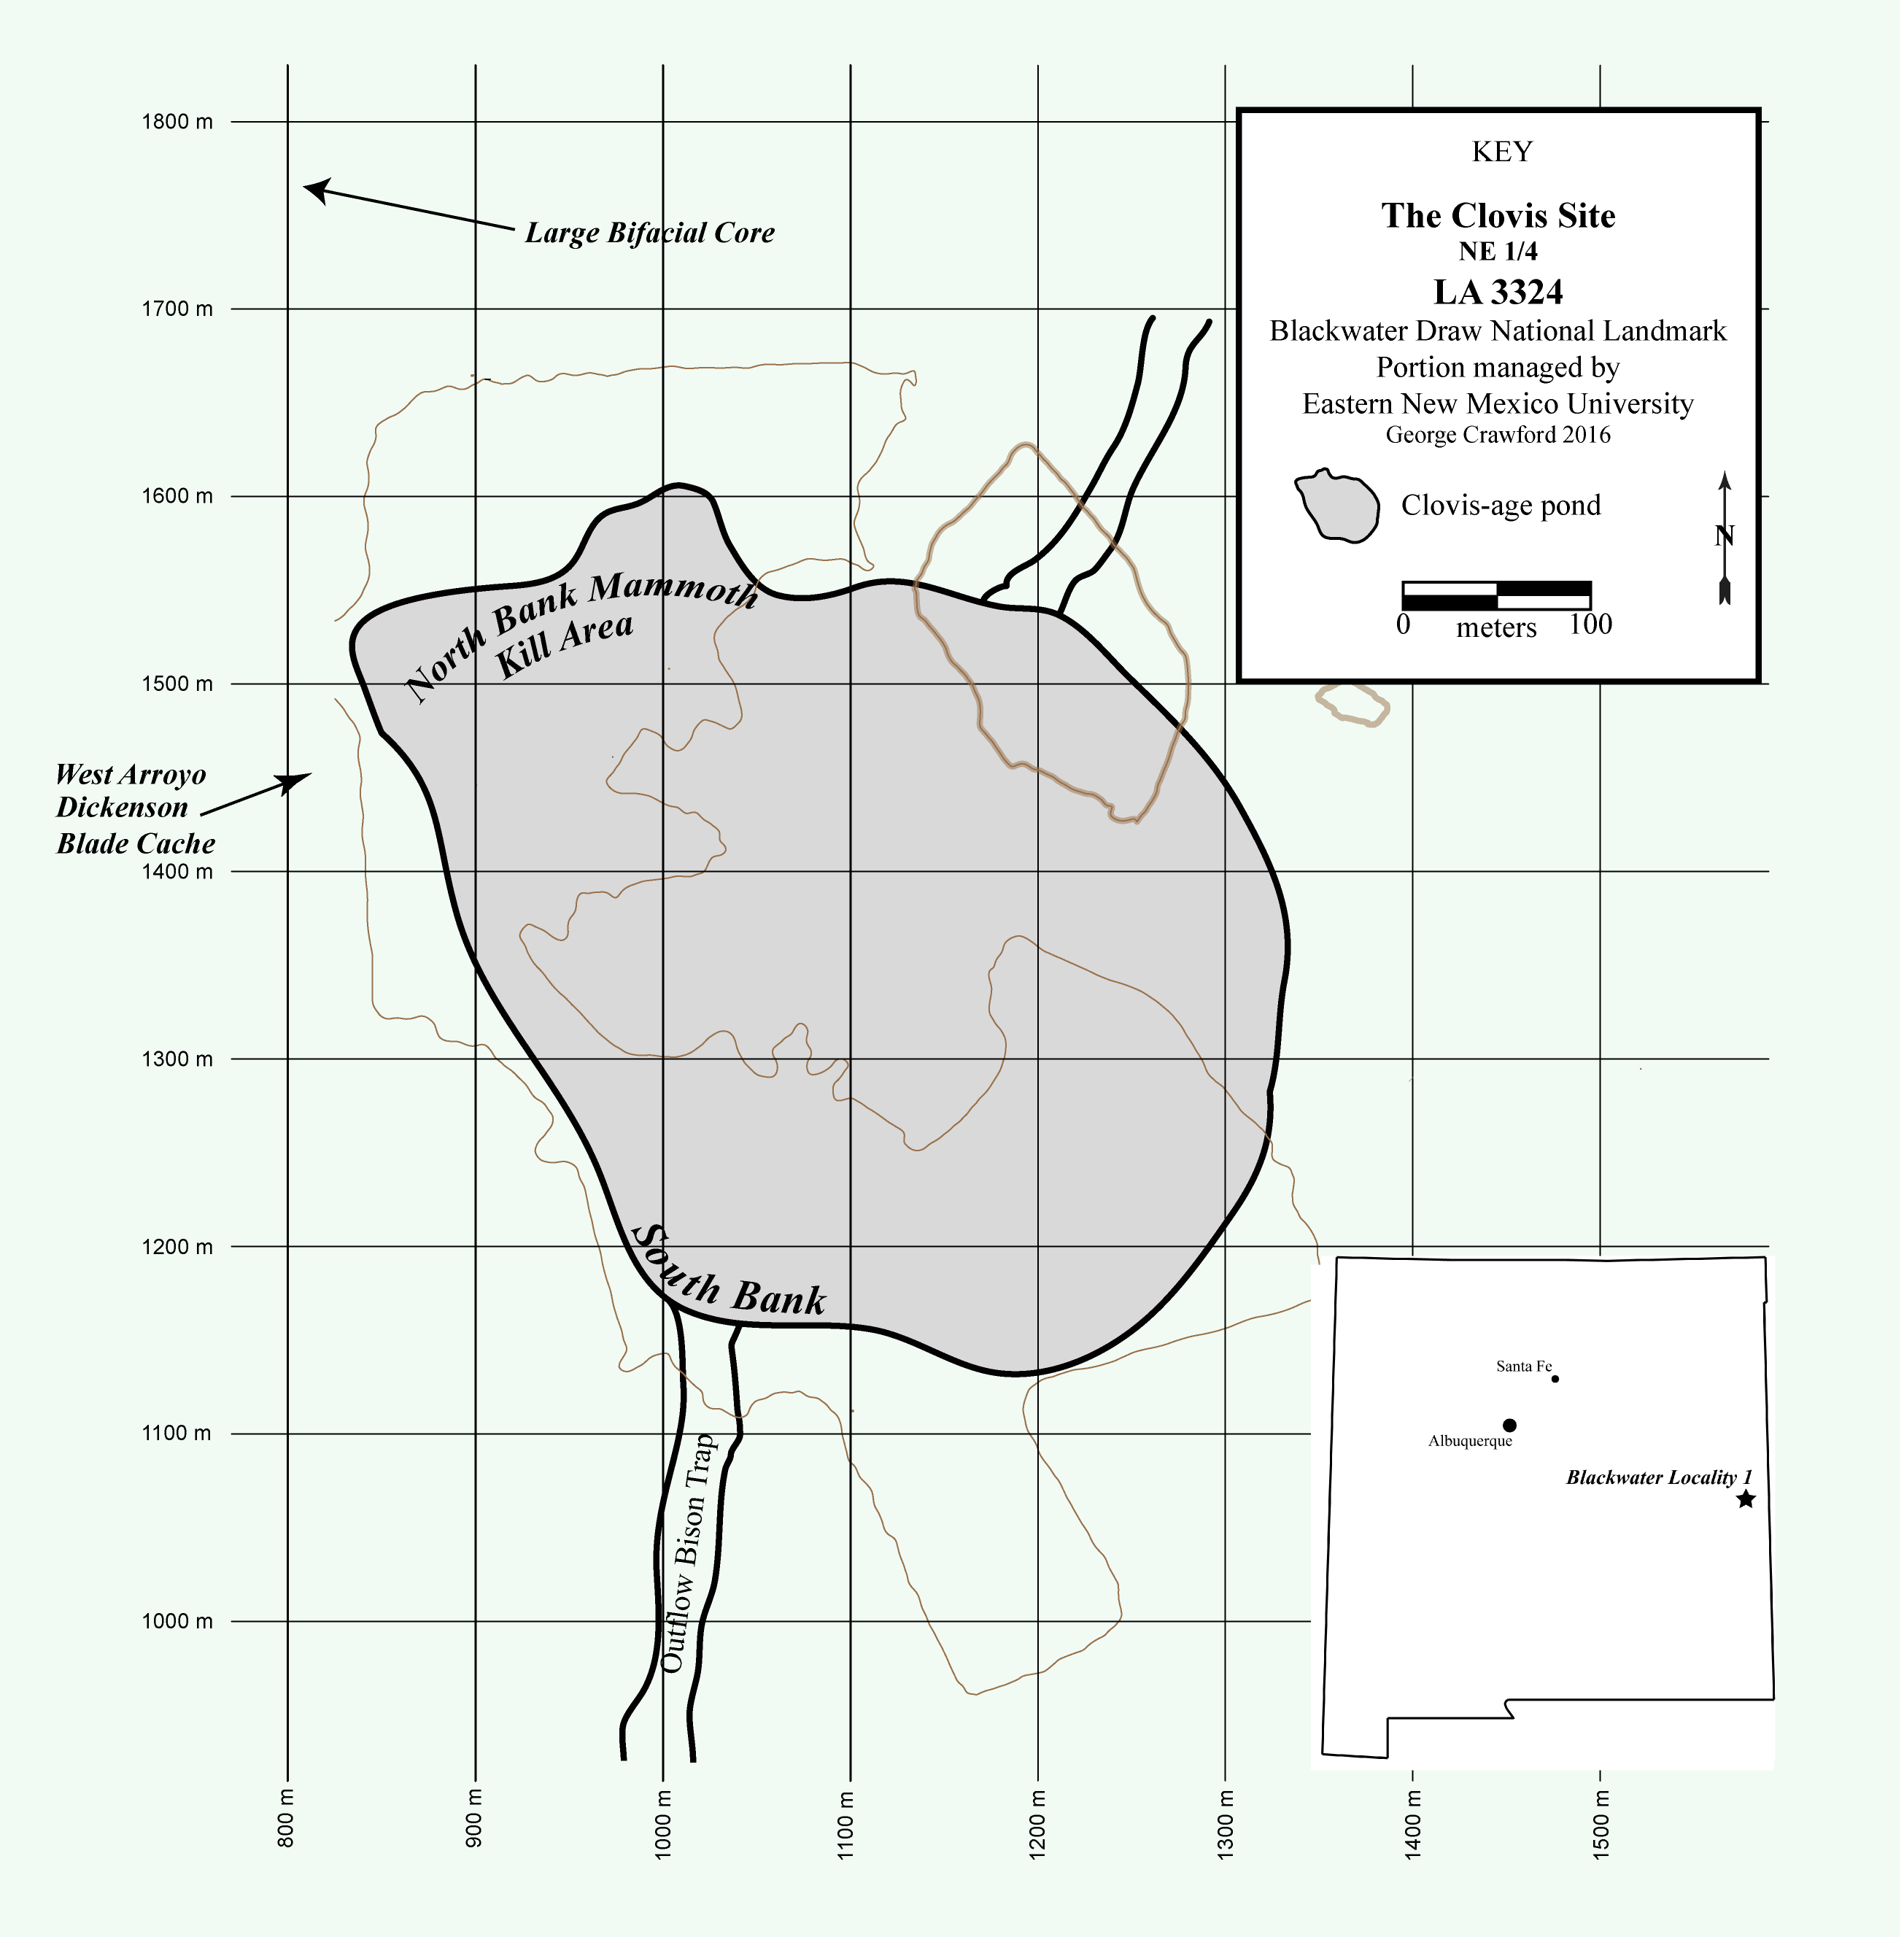
\includegraphics[width=\linewidth]{Fig1}
\caption{Map of NE 1/4 of the Blackwater Draw NHL (LA3324).}
\label{fig:Fig1}
\end{figure}

\begin{figure}[ht]\centering

\includegraphics[width=\linewidth]{Fig2}
\caption{3D scan data for ENMU LA3324 25313. \em This is a 3D figure that can be rotated, measured and otherwise quantified. To activate the figure, this article must be downloaded to your computer. Activate the figure by clicking on the image, then click/drag to rotate.}
\label{fig:Fig2}
\end{figure}

\subsection{Context}

While the detailed context of these artifacts is discussed elsewhere \citep{RN4612, RN4604, RN4605, RN4606, RN4607, RN4609}, an abbreviated listing is included in Table ~\ref{tab:Tbl1}, and in each of the Zenodo entries. Those artifacts from Area C include 24136, 24143, 24152, 24156, 24157, 24158 and 24161. The two artifacts from Area D are 24122 (Mammoth II) and 32095, while the large biface is from Area E. Artifacts 6183/6188 (a refit of 6183 and 6188), 6185 and 6186 are from the Dickenson Cache. Clovis points 25313, 25316 and 25317 were found in context with Agogino's Mammoth IV, and Clovis point 25314 with Agogino's Mammoth I. 

\begin{table}[hbt]
\caption{Context of Scanned Artifacts}
\centering
\begin{tabular}{lll}
\hline
Artifact No. & Description & Provenience \\
\hline
Biface & Lg Biface & S. Bank Locality\\
EL-2-120 & Agate Basin Pt & N. Bank Spring\\
6183/6188 & Blade & W. Arroyo\\
6185 & Blade & W. Arroyo\\
6186 & Blade & W. Arroyo\\
24122 & Clovis Pt & N. Bank Mam. Kill\\
24136 & Clovis Pt & N. Bank Mam. Kill\\
24143 & Clovis Pt & N. Bank Mam. Kill\\
24152 & Clovis Pt & N. Bank Mam. Kill\\
24156 & Clovis Pt & N. Bank Mam. Kill\\
24157 & Clovis Pt & N. Bank Mam. Kill\\
24158 & Clovis Pt & N. Bank Mam. Kill\\
24161 & Clovis Pt & N. Bank Mam. Kill\\
25313 & Clovis Pt & N. Bank Mam. Kill\\
25314 & Clovis Pt & N. Bank Mam. Kill\\
25316 & Clovis Pt & N. Bank Mam. Kill\\
25317 & Clovis Pt & N. Bank Mam. Kill\\
25330 & Clovis Pt & W. Wall\\
32095 & Agate Basin Pt & S. Bank\\
\hline
\end{tabular}
\label{tab:Tbl1}
\end{table}

\subsection{Temporal Coverage} 

A representative sample of 11 radiocarbon dates were selected from those areas of the Blackwater Draw NHL that correspond to the known provenience for artifacts reported herein \cite{RN4612, RN4606, RN4607, RN4609} (Figure ~\ref{fig:BWD1}). The Blackwater Draw NHL is the Clovis type site, and most regularly articulates with the Paleoindian period. 

\begin{figure}[ht]\centering
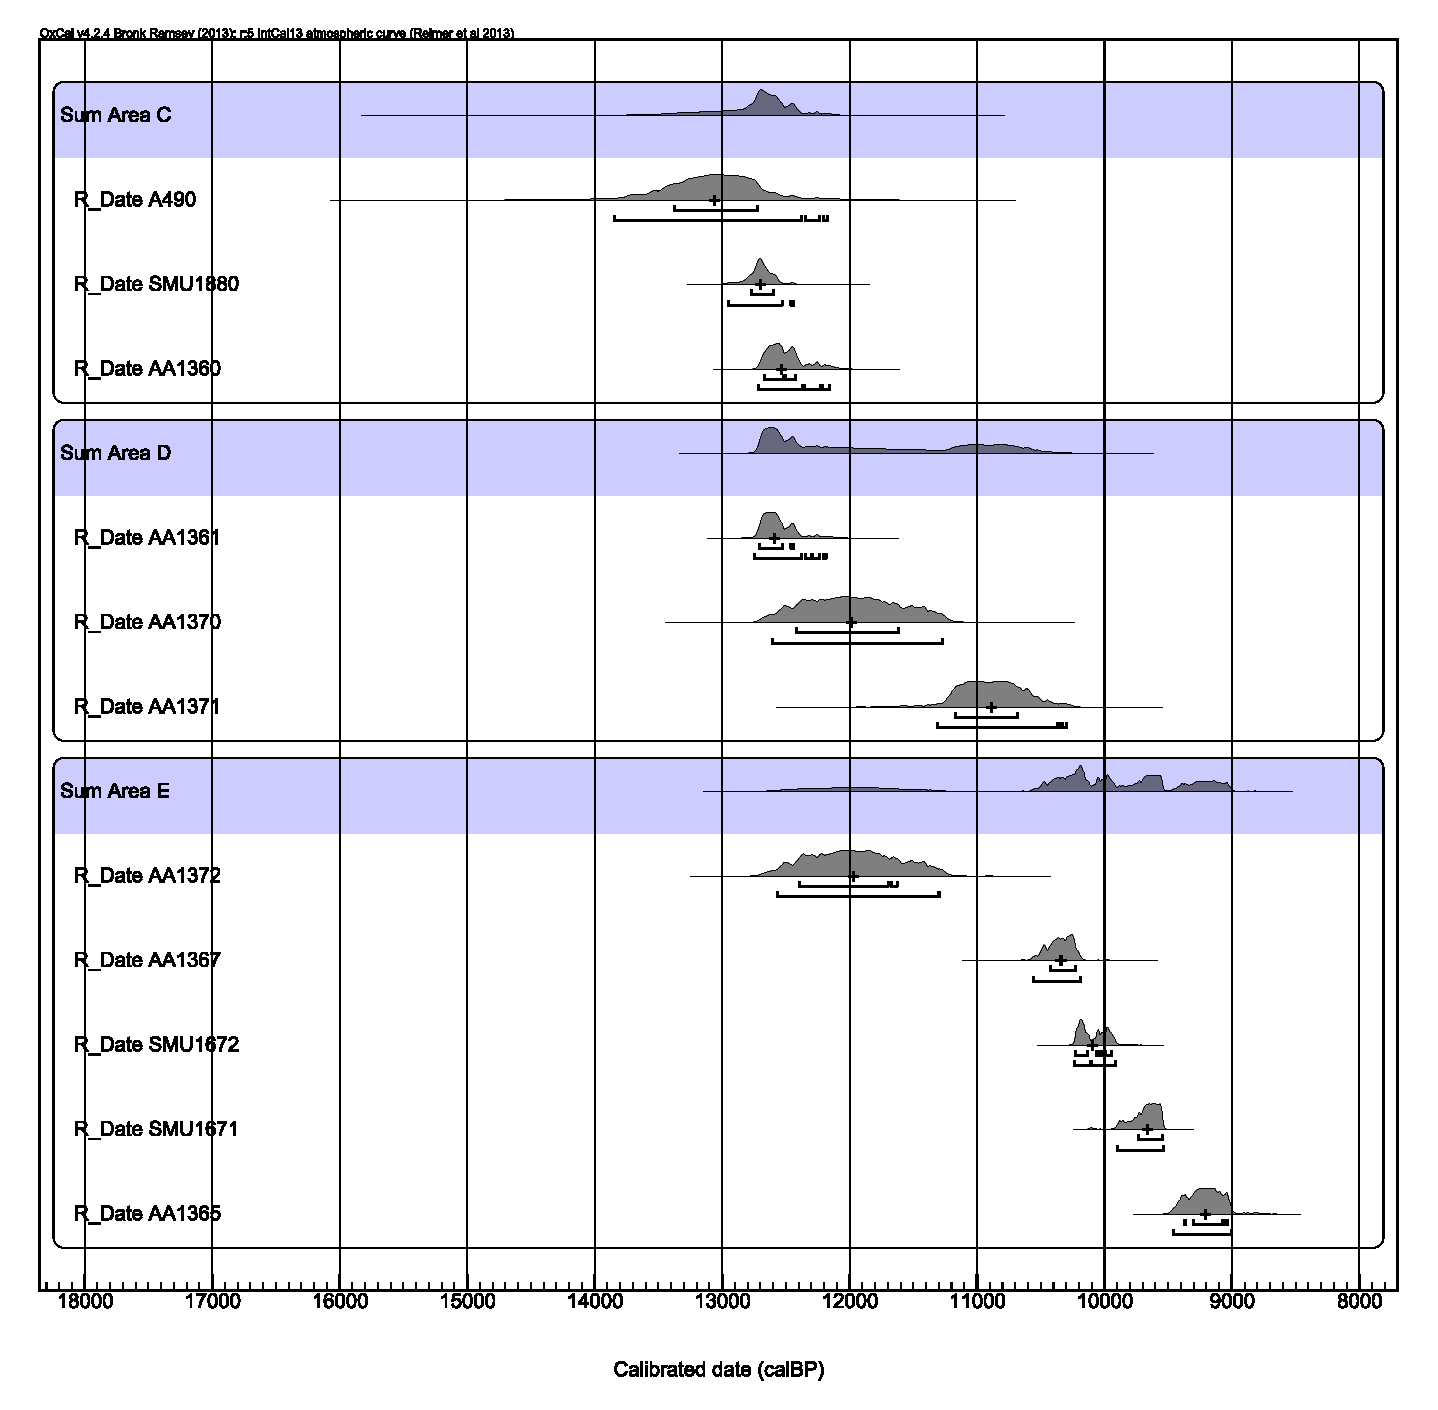
\includegraphics[width=\linewidth]{BWD1}
\caption{Selected radiocarbon dates associated with scanned artifacts from Blackwater Draw NHL. All dates were recalibrated in OxCal \citep{RN308} using the IntCal13 \citep{RN4611} calibration curve.}
\label{fig:BWD1}
\end{figure}

%------------------------------------------------

\section{Methods}

Selected artifacts were scanned using a NextEngineHD running ScanStudioHD Pro. Scan data were collected at the highest HD setting using eight divisions, then trimmed, aligned, fused and polished in ScanStudioHD Pro, before being exported as ASCII.stl and ASCII.ply files prior to post-processing \cite{Galeazzi:1,Weyrich:1}. Those data were then imported into Geomagic Design X, where the final meshes were aligned and processed.

\subsection{Steps}

To align each scan, a reference vector was inserted, followed by a reference point at the confluence of the vector and the mesh (using a projection) at the central base. A plane was then inserted using the pick point and normal axis function, utilizing the vector as the normal axis, and the projected point as the pick point. Both elements (reference vector and reference point) of reference geometry were then utilized in an interactive alignment, with the the reference vector as the moving vector, and the reference point as the moving point (Figure ~\ref{fig:Fig2}). Alignment has proven to be an important factor in downstream analyses, particularly when making the transition from Design X and Control to SolidWorks or other CAD-based platform \cite{Selden:5} (Figure ~\ref{fig:Fig4}). 

\begin{figure}[ht]\centering
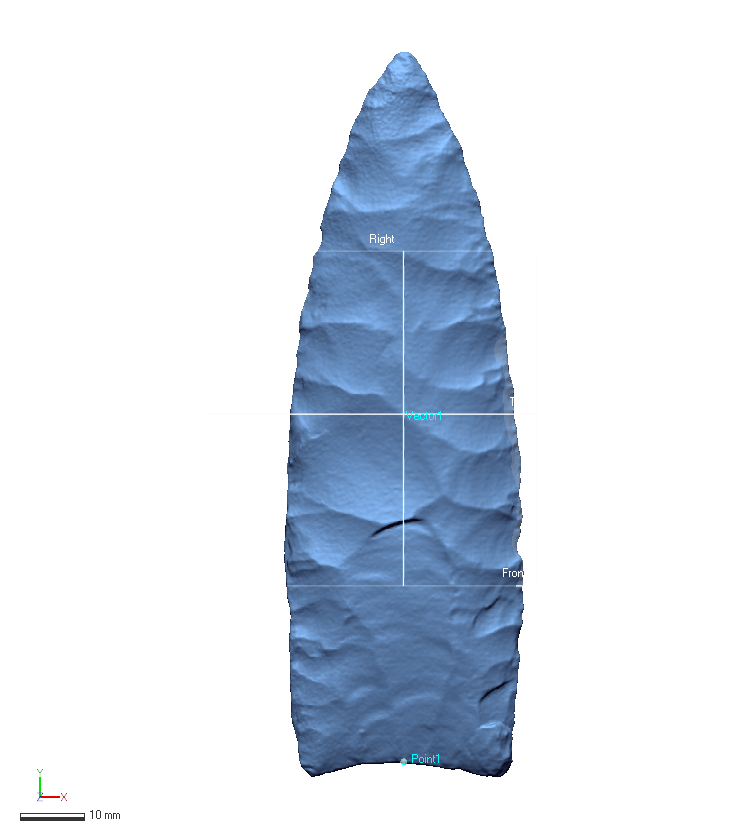
\includegraphics[width=\linewidth]{Fig3}
\caption{Aligned 3D mesh for ENMU LA3324 25313 illustrating the reference geometry (reference vector, point and plane--in green) used to align the mesh.}
\label{fig:Fig3}
\end{figure}

Post-processing of each 3D mesh began with the healing wizard function in Design X, which corrects problematic issues with non-manifold poly-vertices, folded poly-faces, dangling poly-faces, small clusters, small poly-faces, non-manifold poly-faces, crossing poly-faces, and small tunnels. After these issues were corrected, the rewrap function was used to render the final mesh. Upon completion of post-processing, each mesh was decimated by 50 percent prior to saving then export as an ASCII.ply. Decimation of the mesh decreases file size while increasing ease of use on standard computers.

\subsection{3D Puzzles}

In addition to the 3D models, one 3D cardboard puzzle was created (for ENMU LA3324 25313 \cite{Selden:Z}) to augment the on-site efforts of the interpretive staff by providing a physical model through which visitors can interact with the digital proxy. These cardboard puzzles were generated using Autodesk 123D Make \cite{Autodesk:1}, and the plans for the cardboard puzzles (Figure ~\ref{fig:Fig4}) accompanied the uploads to Zenodo. Those plans can be downloaded, glued to cardboard, then cut out to create a tangible model of a Clovis point. These files were uploaded to Zenodo in .pdf format, and are also compatible with most laser cutters.

\begin{figure}[ht]\centering
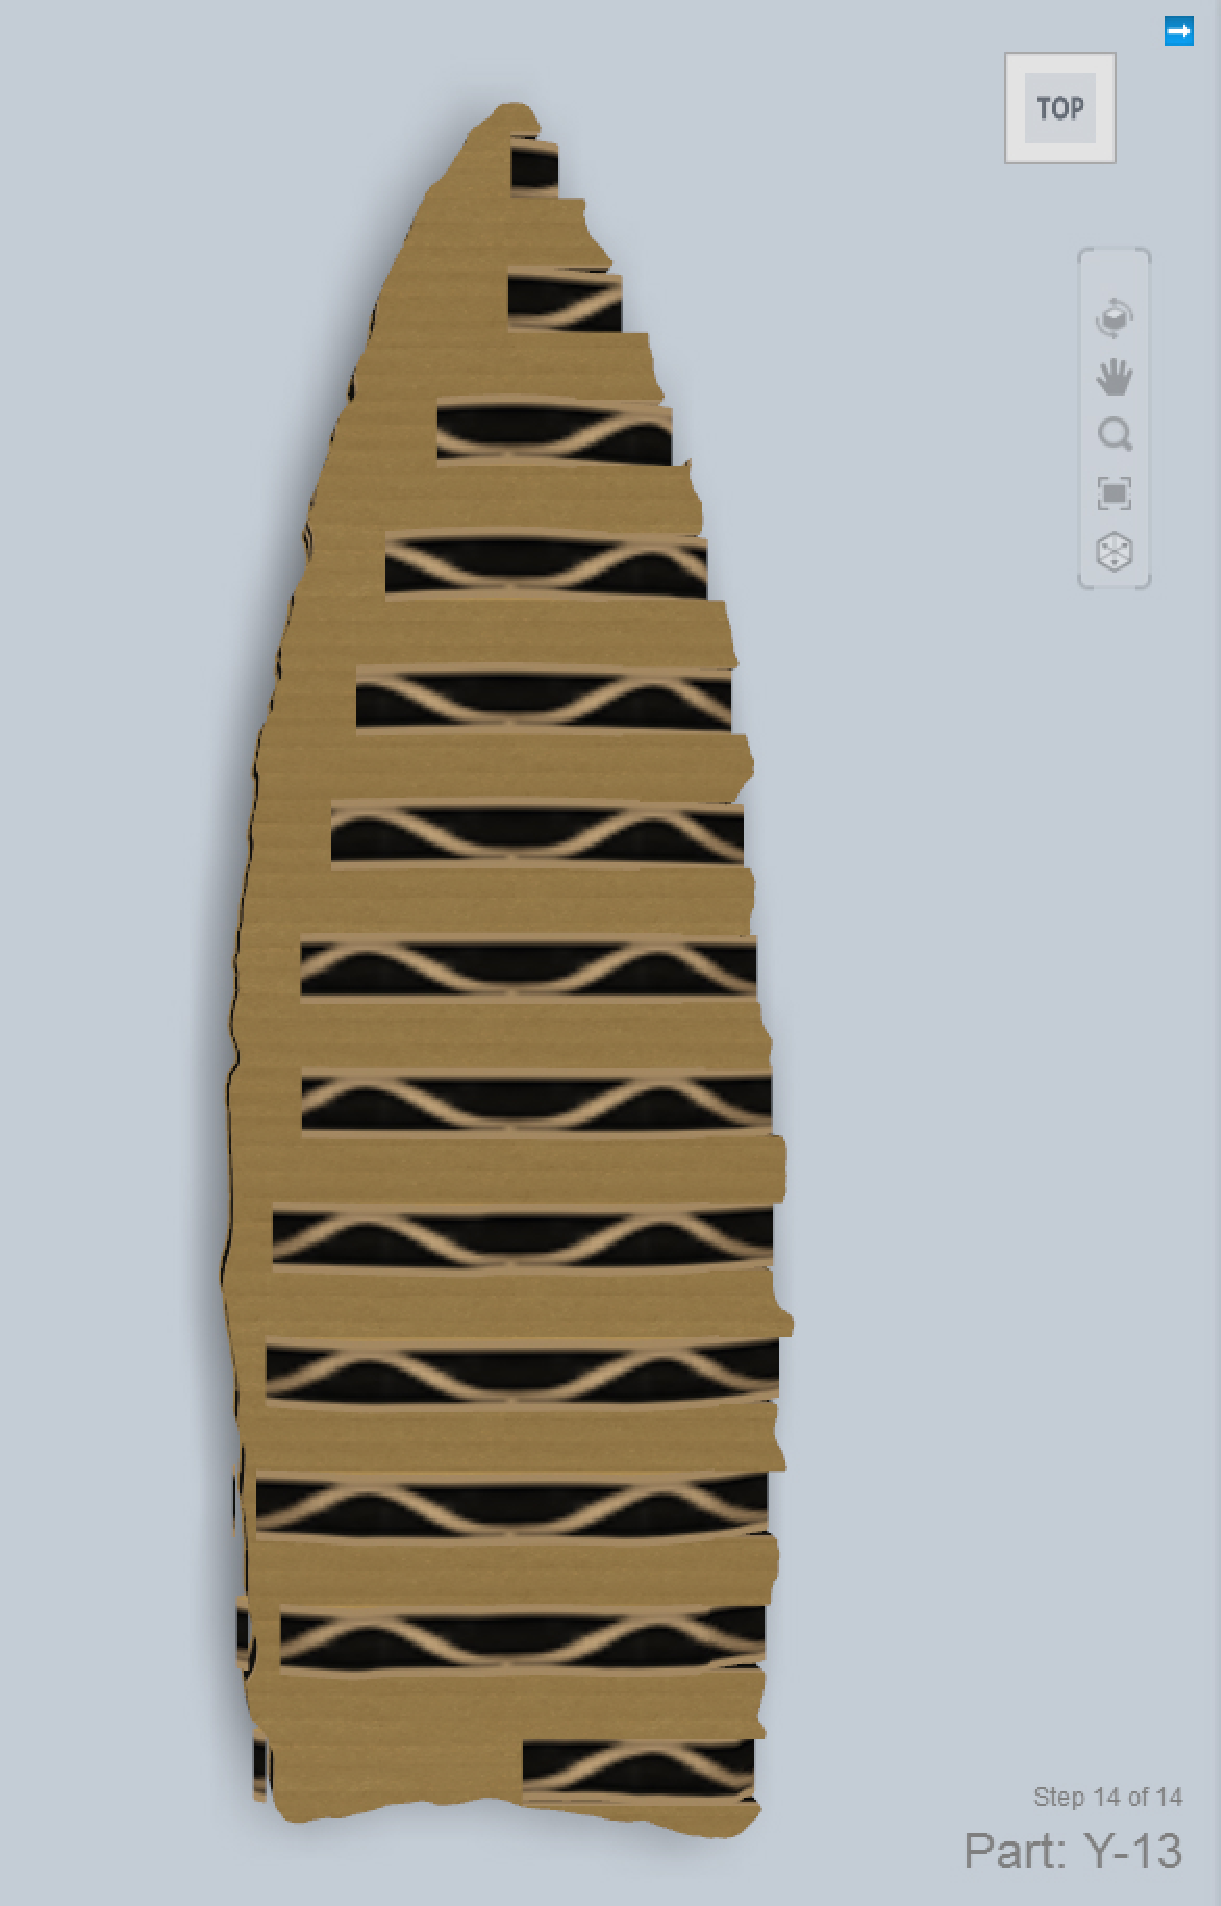
\includegraphics[width=\linewidth]{Fig4}
\caption{Modeled 3D puzzle of ENMU LA3324-25313 created with Autodesk 123D Make.}
\label{fig:Fig4}
\end{figure}

\section{Data Description}

\subsection{Collection Name}

3D Scans from Blackwater Draw National Historic Site

\subsection{Data Type}

Decimated meshes

\subsection{Format Names and Versions}

ASCII.ply (mesh)

\subsection{Creation Dates}

Feb 8-11, 2016

\subsection{Dataset Creators}

Robert Z. Selden Jr.

\subsection{Language}

English

\subsection{License}

Creative Commons Attribution

\subsection{Repository Location}
3D Scans from Blackwater Draw National Historic Site

\begin{itemize}

\item ENMU LA3324 Biface \citep{Selden:Z1}

\item ENMU LA3324 EL-2-120 \citep{Selden:Z2}

\item ENMU LA3324 6183/6188 \citep{Selden:Z3}

\item ENMU LA3324 6185 \citep{Selden:Z4}

\item ENMU LA3324 6186 \citep{Selden:Z5}

\item ENMU LA3324 24122 \citep{Selden:Z6}

\item ENMU LA3324 24136 \citep{Selden:Z7}

\item ENMU LA3324 24143 \citep{Selden:Z8}

\item ENMU LA3324 24152 \citep{Selden:Z9}

\item ENMU LA3324 24156 \citep{Selden:Z10}

\item ENMU LA3324 24157 \citep{Selden:Z11}

\item ENMU LA3324 24158 \citep{Selden:Z12}

\item ENMU LA3324 24161 \citep{Selden:Z13}

\item ENMU LA3324 25313 \citep{Selden:Z14}

\item ENMU LA3324 25314 \citep{Selden:Z15}

\item ENMU LA3324 25316 \citep{Selden:Z16}

\item ENMU LA3324 25317 \citep{Selden:Z17}

\item ENMU LA3324 25330 \citep{Selden:Z18}

\item ENMU LA3324 32095 \citep{Selden:Z19}

\end{itemize}

\subsection{Data Publication Date}

March 3, 2016

\section{Reuse Potential}

Those data from this project have long-term and wide-ranging reuse potential, of which many applications may (likely) not yet have been contemplated. While the primary purpose of this endeavor was to document these resources for use in additional analytical and outreach efforts, one of the projectile points has since been modeled as 3D puzzles that can be cut out using materials that are easily acquired by most (i.e., a cardboard box). 

These data have significant reuse potential in the digital humanities where they can augment both qualitative and quantitative studies. They also hold promise for clarifying questions of the shape, form, size and asymmetry of these artifacts, which can be addressed in analyses of asymmetry and geometric morphometrics. 

\section*{Acknowledgments}

We extend our gratitude to the Blackwater Draw NHL and to Eastern New Mexico University for providing the requisite permissions and access needed to scan this selection of artifacts. We also thank Dr. Michael J. Shott and Dr. Briggs Buchanan for their comments on an earlier draft.

The 3D model used in Figure ~\ref{fig:Fig2} was generated as a .ply in Geomagic Design X and converted to a .u3d in Daz3D.

%% The Appendices part is started with the command \appendix;
%% appendix sections are then done as normal sections
%% \appendix

%% \section{}
%% \label{}

%% References
%%
%% Following citation commands can be used in the body text:
%% Usage of \cite is as follows:
%%   \cite{key}          ==>>  [#]
%%   \cite[chap. 2]{key} ==>>  [#, chap. 2]
%%   \citet{key}         ==>>  Author [#]

%% References with bibTeX database:

\bibliographystyle{model1-num-names}
\bibliography{LA3324.bib}

%% Authors are advised to submit their bibtex database files. They are
%% requested to list a bibtex style file in the manuscript if they do
%% not want to use model1-num-names.bst.

%% References without bibTeX database:

% \begin{thebibliography}{00}

%% \bibitem must have the following form:
%%   \bibitem{key}...
%%

% \bibitem{}

% \end{thebibliography}


\end{document}

%%
%% End of file `elsarticle-template-1-num.tex'.